\documentclass{article}
\usepackage[T1]{fontenc}
\usepackage{lmodern}
\usepackage{graphicx}
\usepackage{amsmath,amssymb}
\usepackage[a4paper,margin=2cm]{geometry}
\usepackage[absolute,overlay]{textpos}
\setlength{\TPHorizModule}{1mm}
\setlength{\TPVertModule}{1mm}
\usepackage[indonesian]{babel}
\usepackage{hyperref}
\setlength{\emergencystretch}{2em}
% unit: Halaman 26

\begin{document}

% === Halaman 26 (python/native) ===

26

(a) 

Teks 


“Kita semua bersaudara” 

“Hello, world!” 

“Namaku Alice” 


(b) Gambar 




(c) Audio 




Sumber: http://cloudinary.com  

(d) Video 




Sumber: http://www.engineersgarage.com

% deskripsi: gambar native xref 135
\noindent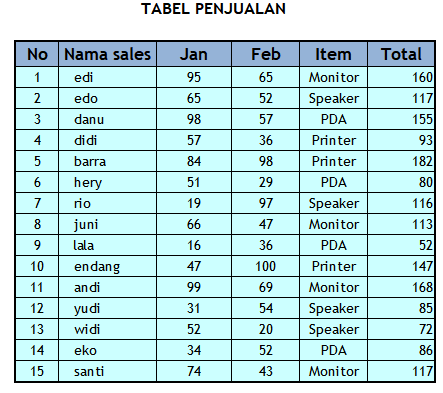
\includegraphics[width=0.85\textwidth]{../../images/python/page_026_img_01.png}

% deskripsi: gambar native xref 136
\noindent
\includegraphics[width=0.85\textwidth]{../../images/python/page_026_img_02.jpeg}

% deskripsi: gambar native xref 132
\noindent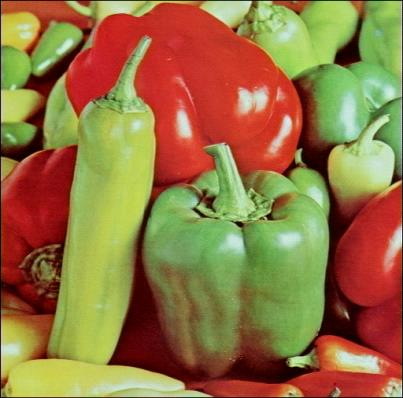
\includegraphics[width=0.85\textwidth]{../../images/python/page_026_img_03.jpeg}

% deskripsi: gambar native xref 133
\noindent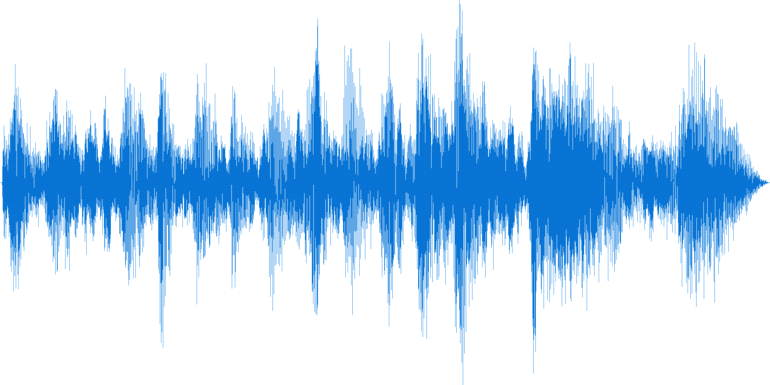
\includegraphics[width=0.85\textwidth]{../../images/python/page_026_img_04.png}

% deskripsi: gambar native xref 134
\noindent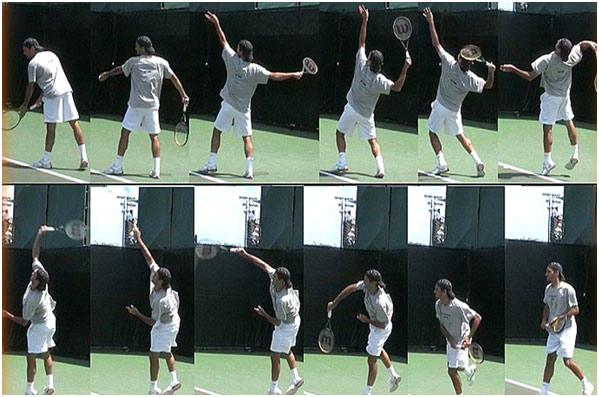
\includegraphics[width=0.85\textwidth]{../../images/python/page_026_img_05.jpeg}

\end{document}
